\chapter{Numbers and Symbols: Turning Specific Problems into Portable Models}

\section{A Hundred-Yuan Shopping List}

The day before school starts, your mother hands you a hundred-yuan note. ``Go and buy the stationery you'll need this term. Notebooks cost six yuan each and gel pens cost four yuan each. Choose the quantities yourself, and try to spend exactly one hundred yuan.''

It sounds like a small errand, but standing before the shelves in the stationery shop, you discover a proper problem: how many notebooks and pens should you buy to spend exactly one hundred yuan? Your mother might even add another condition: ``You need both notebooks and pens. You can't buy just one kind.''

Start with a guess. Ten notebooks cost sixty yuan, leaving forty yuan for exactly ten pens. There is one answer: $10$ notebooks and $10$ pens. Are there other ways? $16$ notebooks cost ninety-six yuan; add one pen and the total is exactly one hundred. There seems to be more than one answer. That raises a more ambitious question:

\begin{center}
\textbf{How many ways are there? Can you guarantee you have missed none and counted none twice?}
\end{center}

This question can leave you stuck. Unlike ``How much do $10$ notebooks and $10$ pens cost?'', it cannot be answered with a single calculation. You have to find \emph{all} the answers and explain why none are missing. Calling out a number on instinct is not enough. You say there are $8$ ways; your classmate says $9$. Who is right? How do you decide?

That is where this chapter begins. We will start by patiently trying arithmetic and see how the work gets out of hand. Then we will introduce our main characters---\emph{algebraic symbols}---and turn ``each individual problem'' into ``a whole class of problems.'' Finally, you will have a small model that solves more than this shop's problem. You can carry it, unchanged, into taxi fares, mobile phone plans, mixing drinks, dividing New Year gift money, and many other situations that seem unrelated.

\section{The Arithmetic Approach: When Trying Every Case Gets Out of Hand}

Anyone can think of the simplest method: try the possibilities one by one.

You must buy at least $1$ notebook and at most $16$ ($17$ would cost more than one hundred yuan). For each number of notebooks, work out the money left, then check whether it is divisible by four with a quotient of at least $1$. We obtain this table:

\begin{center}
\begin{tabular}{ccc}
\toprule
Notebooks $x$ & Money left (yuan) & Gel pens $y$ \\
\midrule
$2$ & $100-12=88$ & $22$ \\
$4$ & $100-24=76$ & $19$ \\
$6$ & $100-36=64$ & $16$ \\
$8$ & $100-48=52$ & $13$ \\
$10$ & $100-60=40$ & $10$ \\
$12$ & $100-72=28$ & $7$ \\
$14$ & $100-84=16$ & $4$ \\
$16$ & $100-96=4$ & $1$ \\
\bottomrule
\end{tabular}
\end{center}

After careful checking, there are $8$ ways in total. Notice one detail: an odd number of notebooks never works. The remaining money would be an amount such as $94$ or $82$ yuan, which leaves a remainder when divided by $4$. You cannot buy a whole number of pens. We discovered this by counting the money case by case.

The problem seems solved. But consider the cost of this method: $16$ subtractions, $16$ divisions, and constant attention to whether the money left can be spent exactly. If your mother changes the budget to one hundred and fifty or two hundred yuan, you must redo the table. If the shop adds another item---stickers at two yuan each, say---and the condition becomes ``buy all three kinds and spend exactly one hundred yuan,'' enumeration no longer fits in a single short table. It takes dozens or even hundreds of rows: the possibilities with $1$ sticker, then with $2$ stickers, and so on. Doing this by hand, an error is only a matter of time.

Arithmetic fails here not because its calculations are wrong, but because \emph{every new problem requires a fresh start}. Solving the hundred-yuan problem leaves us no reusable result for a hundred and twenty yuan; counting combinations of two items gives us no ready method for three. We need more than faster trial and error. We need a way to write down the process of trying itself.

\begin{shiyan}
Take a sheet of paper and repeat the enumeration above with a budget of $120$ yuan. Notebooks still cost $6$ yuan, pens still cost $4$ yuan, and you must buy at least one of each. Count how many divisions you perform. Before reading on, ask yourself: is there a pattern repeated in those divisions? If you had to describe the same pattern to a robot that knew no arithmetic, how would you write it?
\end{shiyan}

\section{A Quick Roll Call: The Numbers We Already Know}

Before bringing algebraic symbols onstage, let's greet some old friends. From this chapter onward, they will often appear together in the same expression.

The \emph{natural numbers} $0,1,2,3,\dots$ are the counting numbers. Counting notebooks or sharing sweets belongs to their territory. The \emph{integers} add the negative numbers $-1,-2,-3,\dots$, which describe quantities in the ``opposite direction'': three degrees below zero, a debt of five yuan, the second basement floor in a lift. Place the integers on a straight line and you get our familiar number line:

\begin{center}
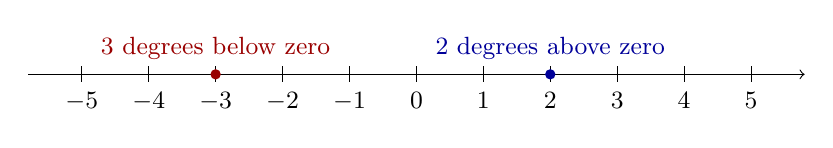
\begin{tikzpicture}[scale=0.85]
\draw[->] (-5.8,0) -- (5.8,0);
\foreach \x in {-5,-4,-3,-2,-1,0,1,2,3,4,5}
  \draw (\x,0.12) -- (\x,-0.12) node[below] {\small $\x$};
\fill[red!60!black] (-3,0) circle (2.2pt) node[above=2pt] {\small $3$ degrees below zero};
\fill[blue!60!black] (2,0) circle (2.2pt) node[above=2pt] {\small $2$ degrees above zero};
\end{tikzpicture}
\end{center}

\emph{Fractions}, together with their close relatives decimals and percentages, deal with parts of a whole. Half a pizza is $\frac{1}{2}$; a six-yuan notebook sold at seventy-five percent of its price costs $6\times 0.75=4.5$ yuan; $60\%$ of a class joins the spring outing. \emph{Ratios} describe the relative sizes of quantities. A map scale of $1:10000$ says that $1$ centimetre on the map represents $100$ metres on the ground. Sharing $12$ chocolates between two people in the ratio $2:1$ means dividing them into $3$ equal portions, with one person taking two portions and the other taking one.

Each kind of number has its own character. Division can take you outside the natural numbers: $7$ divided by $2$ has no natural-number answer. The same is true of the integers. The world of fractions is much broader: adding, subtracting, multiplying, or dividing two fractions (with a nonzero divisor) always gives another fraction. Percentages are just fractions with denominator $100$. Prices described as seventy-five, eighty, or ninety-five percent of the original all tell you what percentage of the original price you must pay.

Why this roll call? Because whenever we write an expression, we must first decide which numbers its quantities are allowed to take. Numbers of stationery items must be natural numbers; temperatures can be integers or fractions; discounts are percentages. \emph{The world of numbers a problem lives in often determines whether it has a solution and how many solutions it has.} If buying ``$3.5$ notebooks'' were allowed, the hundred-yuan problem would suddenly have endlessly many possibilities---but the shop does not sell half a notebook. We will use this point again shortly.

\section{Naming What We Don't Know: Symbols and Algebraic Expressions}

Return to the hundred-yuan list. Each step in our enumeration did the same thing: suppose we buy some number of notebooks, calculate, and then adjust. Long ago, mathematicians realized that instead of repeatedly writing ``suppose we buy some number,'' we could give this as-yet-unknown number a temporary name: a symbol, usually written as a letter.

Call the number of notebooks $x$ and the number of gel pens $y$. The money spent is
\[
6x+4y,
\]
and the requirement to spend exactly one hundred yuan becomes
\[
6x+4y=100.
\]

Pause to look at this line. It accomplishes our first major step: \emph{that entire table and all those divisions have been compressed into one line}. The line makes no particular guess about how many notebooks to buy. It speaks about every possible purchase at once. Has the budget become a hundred and twenty yuan? No need to rethink the problem; replace the right-hand side with $120$: $6x+4y=120$. Have the unit prices changed? Replace $6$ and $4$. The expression's skeleton stays exactly the same.

An expression such as $6x+4y$, made from numbers, symbols representing numbers, and operation symbols, is called an \emph{algebraic expression}.

\begin{shuyu}{Algebraic Expression}
\textbf{Intuitive explanation}: The skeleton left when you replace the changing parts of an arithmetic problem with symbols.\\
\textbf{Formal definition}: An expression joining numbers and symbols that represent numbers through operations such as addition, subtraction, multiplication, division, and powers.\\
\textbf{An example}: With notebooks at $6$ yuan each and pens at $4$ yuan each, the total cost of $x$ notebooks and $y$ pens is the algebraic expression $6x+4y$. Set $x=10$ and $y=10$, and it becomes the ordinary arithmetic calculation $6\times10+4\times10=100$.
\end{shuyu}

A symbol's first role here is to represent an \emph{unknown}: a particular number whose value we do not yet know and must uncover using the conditions. In $6x+4y=100$, $x$ and $y$ are two unknowns. The shop's restriction that ``$x,y$ are both positive integers''---remember how the world of numbers matters---will help narrow the answers to a finite set.

Do not underestimate the step of giving something a name. Mathematicians worked toward it for over a thousand years. Early mathematical texts had no symbolic notation; a problem occupied a whole paragraph of everyday language: ``There is a quantity. Take three times that quantity and add two. The result is fifty. What is the quantity?'' Before calculating, the reader had to decipher the prose. Mathematicians in different places invented their own abbreviations and marks, could not read one another's ``codes,'' and circulated many arguments about which notation was more convenient. Only as letter notation gradually became standardized could the same problem be compressed into the seven symbols $3x+2=50$. The triumph of notation was not about saving ink. Once all the conditions live in an expression, reasoning can operate directly on that expression without relying on a mental ledger. Every transformation, solution, and generalization later in this chapter benefits from that triumph.

Writing conditions with symbols has another immediate benefit: we can \emph{reason} directly with expressions instead of repeatedly counting money. Consider why an odd number of notebooks is impossible. The expression $6x+4y$ is always even: $6x$ is even, $4y$ is even, and their sum is even. Since $100$ is also even, parity alone gives no contradiction. But the remainder when $6x$ is divided by $4$ depends on $x$. For odd $x$, $6x$ takes values such as $6,18,30$, each a multiple of $4$ plus $2$. Adding $4y$ leaves remainder $2$, whereas $100$ leaves remainder $0$: a contradiction. Thus $x$ must be even. A short argument replaces the eight crossed-out attempts in the table.

\section{The Rules of the Balance: Transforming Equations and Finding a Unique Solution}

Writing $6x+4y=100$ is only the beginning. We must also know how to solve it. First, let's get the terminology straight:

\begin{dingyi}[Equation]
An equality containing unknowns is called an \emph{equation}. Values of the unknowns that make its two sides equal are called \emph{solutions}; finding them is called \emph{solving the equation}.
\end{dingyi}

All the techniques of solving equations rest on an old and simple picture: a balance.

An equality is like a balanced scale. The left pan holds $6x+4y$, the right pan holds $100$, and the beam is level. We can perform the same operation on both sides without upsetting the balance: add equal weights, remove equal weights, double both loads, or halve them. The balance is preserved throughout.

\begin{center}
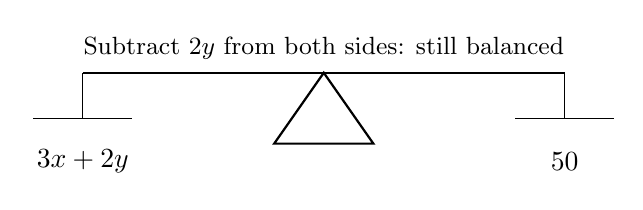
\begin{tikzpicture}[scale=0.9]
\draw[thick] (-0.7,0) -- (0.7,0) -- (0,1.0) -- cycle;
\draw[thick] (-3.4,1.0) -- (3.4,1.0);
\draw (-3.4,1.0) -- (-3.4,0.35);
\draw (3.4,1.0) -- (3.4,0.35);
\draw (-4.1,0.35) -- (-2.7,0.35);
\draw (2.7,0.35) -- (4.1,0.35);
\node at (-3.4,-0.25) {$3x+2y$};
\node at (3.4,-0.25) {$50$};
\node at (0,1.35) {\small Subtract $2y$ from both sides: still balanced};
\end{tikzpicture}
\end{center}

\begin{dingli}[The Balance Principle]
If two expressions are equal, they remain equal when we add or subtract the same number or expression on \emph{both} sides, multiply \emph{both} sides by the same number, or divide \emph{both} sides by the same nonzero number.
\end{dingli}

This principle sounds unremarkable, but it is the constitution of the world of equations. Divide both sides of $6x+4y=100$ by $2$ to obtain the cleaner $3x+2y=50$. Then ``remove'' $2y$ from both sides by subtracting it, giving $3x=50-2y$. Divide by $3$: $x=\dfrac{50-2y}{3}$. Each step merely rearranges the balance while keeping it level. By the end, $x$ has almost been singled out: choose $y$ and you can immediately calculate $x$. Our table repeatedly uses this expression for $y=22,19,16,\dots$.

The classic setting for the balance principle is a linear equation in one unknown: an equation with just one unknown, appearing only to the first power. There is a particularly clean result:

\begin{dingli}[The Solution of a Linear Equation in One Unknown]
Let $a\neq 0$, and let $b,c$ be any known numbers. Then the equation $ax+b=c$ has exactly one solution,
\[
x=\frac{c-b}{a}.
\]
\end{dingli}

\begin{proof}
There are two steps: first find a solution, then show there cannot be a second one.

First, use the balance principle to isolate $x$. Subtract $b$ from both sides to get $ax=c-b$. Since $a\neq0$, divide both sides by $a$, giving $x=\dfrac{c-b}{a}$. Substitute this value into the original equation to check it: $a\cdot\dfrac{c-b}{a}+b=(c-b)+b=c$. The equality holds, so this is a solution.

Second, prove uniqueness. Suppose $x_1$ and $x_2$ both solve the equation, so $ax_1+b=c$ and $ax_2+b=c$. Subtract the equalities, removing equal quantities from the two pans, to obtain $a(x_1-x_2)=0$. Since $a\neq0$, and a product is zero only if at least one factor is zero, we have $x_1-x_2=0$, hence $x_1=x_2$. The supposed two solutions are the same. This completes the proof.
\end{proof}

Notice a small but essential detail: before dividing by $a$, we must establish $a\neq0$. The rule allowing division by the same number has a condition: that number cannot be zero. Division by zero is undefined, so the balance rule has a clear boundary here. This is no mere quibble. When $a=0$, the equation becomes $0\cdot x+b=c$. If $b=c$, every $x$ works; if $b\neq c$, there is no solution. Neither case has exactly one solution. \emph{A theorem's conditions are as much a part of it as its conclusion.}

Here is a numerical example of the theorem's power. The stationery shop offers two promotions. Plan A takes twenty-five yuan off purchases of at least one hundred yuan; Plan B charges seventy-five percent of the original price. At what purchase amount do they offer equal savings? Let the original price be $x$ yuan, assuming $x\geq100$ so Plan A applies. You pay $x-25$ yuan under A and $0.75x$ yuan under B. Equal savings means $x-25=0.75x$. Subtract $0.75x$ to get $0.25x=25$, then divide by $0.25$: $x=100$. They tie at exactly one hundred yuan; beyond that, B is cheaper because its discount grows with the total, while A's reduction stays fixed. Percentages, linear equations, and the balance principle have worked together on an everyday problem.

\section{The World Is Not Always Exact: Inequalities}

If your mother relaxes her instruction to ``buy what you like within one hundred yuan, but don't overspend,'' an equality no longer captures it. The amount $6x+4y$ need not equal a fixed number; it must satisfy
\[
6x+4y\leq 100.
\]
This is an \emph{inequality}. Most real-world constraints look like this: stay within a budget, finish before a deadline, keep below a weight limit, or score at least a passing grade. Equalities describe an exact fit; inequalities describe an acceptable range. The latter territory is much larger.

Inequalities can also be transformed, but their rules come with an extra warning. Adding or subtracting the same number on both sides preserves the direction. Multiplying or dividing by a \emph{positive} number preserves it too. But multiplying or dividing by a \emph{negative} number requires reversing the inequality sign.

Why? One look at the number line explains it. $2<3$ means $2$ lies to the left of $3$. Multiplying both sides by $-1$ gives $-2$ and $-3$, reflected across $0$. Now $-2$ lies to the \emph{right} of $-3$, so $-2>-3$. Multiplication by a negative number mirrors the number line, exchanging left and right.

\begin{fanli}
Alert one: ``Multiplying both sides of an inequality by the same number preserves its direction.'' Wrong. Try multiplying by $-1$. Starting with $5<7$, it would be absurd to conclude $-5<-7$; the correct result is $-5>-7$. Only a \emph{positive} multiplier preserves direction. A negative multiplier reverses it, and multiplying by zero turns both sides into $0$, making the strict inequality collapse.

Alert two: ``An algebraic symbol represents a hidden unknown and becomes useless once you solve for it.'' Also wrong. In $6x+4y=100$, $x,y$ can take $8$ different pairs of values; the symbols represent all the candidates. In the next section, you will see symbols stand for any natural number. Thinking of a symbol only as one concealed number misses much of its power.
\end{fanli}

Inequalities and equalities often work together. Return to the three-item problem: notebooks at $6$ yuan, pens at $4$ yuan, stickers at $2$ yuan, buying all three kinds and spending exactly one hundred yuan. If we buy $z$ stickers, the first two quantities must satisfy $6x+4y=100-2z$, with $x\geq1$ and $y\geq1$. Those inequalities limit $z$: $100-2z$ must cover at least one notebook and one pen, so $100-2z\geq10$, giving $z\leq45$; also $z\geq1$. Thus $z$ ranges only from $1$ to $45$. For each $z$, solve a two-unknown problem we already understand. Inequalities have trimmed a daunting three-unknown enumeration into a bounded task we can handle in batches.

\section{Another Job for Symbols: Representing a Whole Class of Numbers}

So far, symbols have stood for particular numbers that are not yet known. But they have a second, perhaps more important job: speaking about \emph{all} numbers at once.

Consider an old pattern. What is the sum of the natural numbers from $1$ to $100$? Brute force requires $99$ additions. Legend says that the young Gauss answered $5050$ within seconds in class. The story's details may have been embellished, but its underlying idea is sound, and symbols express it in a single sentence.

\begin{dingli}[The Sum of Consecutive Natural Numbers]
For every positive integer $n$,
\[
1+2+3+\cdots+n=\frac{n(n+1)}{2}.
\]
\end{dingli}

\begin{proof}
Write the sum twice, once forward and once backward, with the terms aligned:
\[
\begin{array}{ccccccc}
1 & + & 2 & + \cdots + & (n-1) & + & n\\
n & + & (n-1) & + \cdots + & 2 & + & 1
\end{array}
\]
Each vertical pair sums to $n+1$: first $1+n$, then $2+(n-1)$, and so on, ending with $n+1$. There are $n$ pairs, so the two rows together total $n(n+1)$. They are two copies of the same sum, hence
\[
2\bigl(1+2+\cdots+n\bigr)=n(n+1),
\]
and dividing both sides by $2$ using the balance principle gives the result. This completes the proof.
\end{proof}

Substitute $n=100$: $\dfrac{100\times101}{2}=5050$, just as in the legend. But the theorem says much more than how to add from $1$ to $100$. It works when $n$ is $7$, $1000$, or $1000000$. \emph{One symbol, $n$, combines infinitely many addition problems into one.} That is a symbol's second job: representing any member of an entire class of numbers, rather than one unknown.

The formula also has a geometric face. Picture $1+2+\cdots+n$ as an arrangement of dots: $1$ in the first row, $2$ in the second, and so on to $n$ in the last, forming a triangle. Take two identical dot triangles and turn one over. Together they form a rectangle with $n$ rows and $n+1$ columns:

\begin{center}
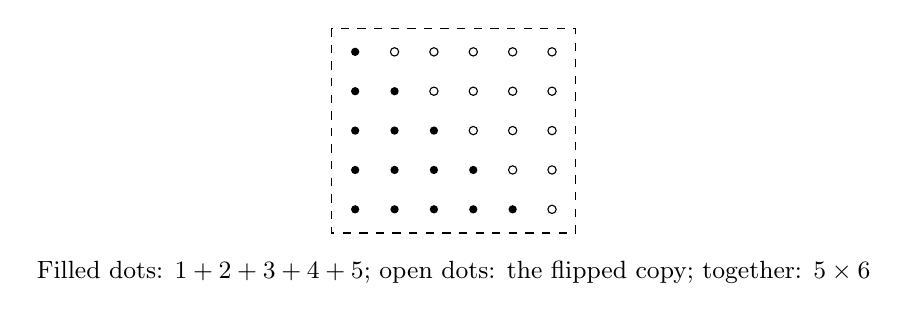
\begin{tikzpicture}[scale=0.5]
\foreach \j in {1} \fill (\j,-1) circle (3pt);
\foreach \j in {1,2} \fill (\j,-2) circle (3pt);
\foreach \j in {1,2,3} \fill (\j,-3) circle (3pt);
\foreach \j in {1,2,3,4} \fill (\j,-4) circle (3pt);
\foreach \j in {1,2,3,4,5} \fill (\j,-5) circle (3pt);
\foreach \j in {2,3,4,5,6} \draw (\j,-1) circle (3pt);
\foreach \j in {3,4,5,6} \draw (\j,-2) circle (3pt);
\foreach \j in {4,5,6} \draw (\j,-3) circle (3pt);
\foreach \j in {5,6} \draw (\j,-4) circle (3pt);
\foreach \j in {6} \draw (\j,-5) circle (3pt);
\draw[dashed] (0.4,-0.4) rectangle (6.6,-5.6);
\node at (3.5,-6.6) {\small Filled dots: $1+2+3+4+5$; open dots: the flipped copy; together: $5\times6$};
\end{tikzpicture}
\end{center}

In the proof, we wrote the sum twice and paired the terms. In the picture, we took two copies and made a rectangle. Algebra states a fact and geometry states it again. This habit of expressing the same idea in two ways will return throughout the book.

\begin{shuyu}{Variables, Parameters, and Constants}
\textbf{Intuitive explanation}: Three roles in a play. Variables are the actors who move; parameters are scenery fixed for one performance but replaceable for another; constants are props that never change.\\
\textbf{Formal definition}: A quantity that can take different values within a problem is a variable. A quantity held fixed for a given problem but allowed to change between related problems is a parameter. A number that does not change is a constant.\\
\textbf{An example}: In $6x+4y=100$, $x,y$ are variables and $6,4,100$ are constants. Generalize to $px+qy=m$, with prices $p,q$ and budget $m$. Then $x,y$ remain variables, while $p,q,m$ are parameters. Changing the shop or the budget changes a set of parameters while leaving the model intact.
\end{shuyu}

Distinguishing these three roles is a key step from solving one problem to building a model. Writing $6x+4y=100$ addresses your mother's particular list. Writing $px+qy=m$ addresses the same kind of problem for \emph{all} prices and \emph{all} budgets. Parameters let a model travel farther.

\section{A Different Perspective: Models Can Travel}

Looking back, this chapter has done one thing: translate a specific problem into a model made of symbols, equalities, and inequalities. The same model repeatedly appears in very different settings. This is what makes algebra so rewarding.

A taxi fare: the initial charge is $10$ yuan, followed by $2$ yuan per kilometre. For a journey of $x$ kilometres, with $x\geq3$ and the first $3$ kilometres covered by the initial charge, the fare is $2(x-3)+10$, or $2x+4$ yuan. With only $30$ yuan, how far can you go? Solve $2x+4\leq30$ to get $x\leq13$. A mobile phone plan: a monthly fee of $19$ yuan includes $10$ GB of data, with additional data charged at $3$ yuan per GB. With a monthly spending limit of $50$ yuan, how much data can you use? Let the extra amount be $x$ GB. Then $19+3x\leq50$, giving $x\leq\frac{31}{3}$, or at most $10$ whole extra GB. Mixing a drink: concentrate and water are mixed in the ratio $1:5$. How much concentrate makes $1.2$ litres? If the concentrate is $x$ litres, then $x+5x=1.2$, so $x=0.2$ litres.

See the common thread? Strip away the details of fares, data, and drinks, and each involves a quantity of the form $ax+b$ with an equality or inequality. The balance rules you learned in the stationery shop work just as well in the taxi, the phone plan, and the kitchen, without changing a word.

Here is the sentence this chapter most wants you to take away: \emph{algebra is not about calculating one problem faster; it is about solving many similar problems at once}. Enumeration grows with the size of the problem: double the budget and the table doubles. The effort of building a model is spent once; each new problem becomes a routine matter of changing parameters and solving an equation. Arithmetic asks for this problem's answer. Algebra asks what the answers to a whole class of problems look like. Moving from one case to a class is exactly what ``portable'' means in this chapter's title.

\begin{lianjie}
This ability to translate is one of the modern world's fundamental technologies. Navigation software turns a road network into constraints between variables and solves an enormous ``how do I arrive fastest?'' problem. Online shopping systems turn stock levels, coupons, and discount rules into hundreds or thousands of expressions like $6x+4y\leq100$, automatically deciding whether an order can go through and what to charge. Every variable you declare in a program is an electronic incarnation of this chapter's algebraic symbols. Each later chapter adds another language to this translator: Chapter 2 adds change, Chapters 3 and 4 add shape, and later come randomness and infinity.
\end{lianjie}

We should also state a model's boundaries honestly. Compressing a taxi journey into $2x+4$ ignores traffic and detours. Comparing discounts through $x-25$ and $0.75x$ assumes you really will spend at least one hundred yuan. \emph{A model translates reality, and every translation involves choices.} A good model captures the main structure and omits irrelevant details. Judging those choices is a shared task for modelers and mathematicians. Chapters 2 and 18 will revisit it.

\begin{pandeng}
Every thread in this chapter leads to a larger world. Equations whose unknowns must be integers, such as the stationery-shop version of $6x+4y=100$, are called \emph{Diophantine equations}. They are a classic hunting ground of number theory, which Chapter 13 will visit. Using inequalities to define a feasible region and finding the best plan within it is the domain of \emph{linear programming}, used daily in operations research and economics to allocate real goods and money. Even the rule that matching operations preserve balance is distilled into the axioms of groups and fields in university \emph{abstract algebra}. Mathematicians ask: what other worlds have balances of their own? Keywords: Diophantine equations, linear programming, axiomatization.
\end{pandeng}

\begin{toolbox}
Keep the new tools from this chapter:
\begin{itemize}
\item \textbf{Introduce symbols}: Name an unknown number or an arbitrary member of a class of numbers. This is the first step in modeling.
\item \textbf{Algebraic expressions}: Isolate what changes and retain a reusable skeleton, such as $6x+4y$.
\item \textbf{The balance principle}: Adding, subtracting, multiplying, or dividing equally on both sides preserves equality, provided the divisor is nonzero. This underlies equation solving.
\item \textbf{Transforming inequalities}: Reverse the sign when multiplying or dividing by a negative number. Equalities describe exact matches; inequalities describe ranges. They often work together.
\item \textbf{Distinguish roles}: Variables vary, parameters change between problems, and constants stay fixed. Parameters make models portable.
\item \textbf{Ask which numbers are allowed}: Must unknowns be natural numbers, integers, or unrestricted numbers? This determines how many solutions there are, or whether any exist.
\end{itemize}
\end{toolbox}

\section*{Reflection Questions}

\textbf{Observation}

\begin{sikao}
\item Look again at the hundred-yuan solutions: $(x,y)=(2,22),(4,19),(6,16),\dots$. Moving to the next purchase increases $x$ by $2$ and decreases $y$ by $3$. Why precisely ``add $2$, subtract $3$''? (Hint: changing the purchase must leave $6x+4y$ unchanged. Increase $x$ and calculate how $y$ must respond.)
\item Plot several pairs $(x,y)$ satisfying $6x+4y\leq100$, with $x\geq1$ and $y\geq1$. Put $x$ horizontally and $y$ vertically, so each purchase becomes a point. What do you notice about their arrangement? (Hint: first plot the points satisfying $6x+4y=100$, then see which side the other points lie on.)
\end{sikao}

\textbf{Proof}

\begin{sikao}
\item Prove that the sum of any two consecutive integers is odd. (Hint: call the smaller integer $n$, express the other using $n$, and add.)
\item Prove $1+3+5+\cdots+(2n-1)=n^2$: the sum of the first $n$ odd numbers is a perfect square. (Hint: imitate the proof that writes the sum twice and pairs terms, or draw dots and add an L-shaped layer around the corner at each step.)
\end{sikao}

\textbf{Challenge}

\begin{sikao}
\item The three-item problem is $6x+4y+2z=100$, with $x,y,z$ positive integers. Design a counting procedure that misses nothing and counts nothing twice, then find the total number of purchases. (Hint: fix $z$ first and return to the two-unknown case solved in this chapter. What conditions must the right-hand side of $6x+4y=100-2z$ satisfy for solutions to exist?)
\item Use $40$ metres of fencing to enclose a rectangular vegetable plot against a wall. The wall forms one side, so only three sides need fencing. Both dimensions must be whole numbers of metres. What arrangement maximizes the area? (Hint: let the side parallel to the wall be $x$ metres and each other side be $y$ metres. Use the fencing length to relate $x,y$, express the area using $x$ alone, and try values in a table. How might the answer change without a wall?)
\end{sikao}

\section*{The Door to the Next Chapter}

The final challenge hides a question this chapter's tools cannot fully answer. With the fencing length fixed, $x$ and $y$ are tied together. Every change in $x$ forces $y$ to change, and the area $S$ changes too. We found a largest area by trying values in a table, but something still feels uncertain. What about nonintegers? Could $x=13.5$ metres be better? We tried a few points and claimed to see the whole picture.

This chapter has focused on individual numbers. But the real subject here is \emph{change itself}: how $S$ rises and falls continuously as $x$ varies. Mathematicians have a new tool for this kind of question: draw the relationship on coordinate paper. The horizontal direction represents $x$ and the vertical direction $S$. Each possible arrangement becomes a point, and together the points form a portrait of the relationship. The portrait shows the highest point, the uphill approach, and the downhill direction. We no longer need to guess or worry about missing intermediate values such as $13.5$.

This portrait is the graph of a \emph{function}. Translating the same relationship from an expression into a picture raises a new set of questions. Why is the graph a parabola? What does its steepness tell us? What does the intersection of two graphs mean? In Chapter 2, we move from solving an equation to studying the shape formed by all its answers.
